\documentclass{article}
\usepackage{anyfontsize}
\usepackage[UTF8]{ctex} % 如果需要支持中文
\usepackage{fontspec} 
    % \setCJKmainfont{SourceHanSansCN-Light}[
    %     BoldFont=SourceHanSansCN-Medium
    % ]

\usepackage[a4paper, left=0.1in, right=0.1in, top=0.05in, bottom=0.05in]{geometry} % 设置四边页边距为0.1英寸{geometry} % 设置页边距为0.5英寸
\usepackage{enumitem} % 用于自定义列表
\usepackage{amsmath}  % 数学公式支持
\usepackage{tikz}
\usetikzlibrary{arrows.meta, positioning}
\setlength{\parindent}{0pt} % 不缩进
\usepackage{etoolbox} % 用于列表操作
%调整类代码
\usepackage{comment}
\usepackage{tocloft} % 用于定制目录 样式
\usepackage{hyperref} %不需要目录盒子注释这
\usepackage{ifthen}
\usepackage{tikz}
\usetikzlibrary{arrows.meta}
\usepackage{titletoc}
\usepackage{graphicx}
\usepackage{float}

\usepackage{amssymb}  % 提供数学符号，包括\therefore
%目录设定
%快捷键 CMD + / 注释
%  \renewcommand{\cftdot}{} % 隐藏目录中的页码
%  \cftpagenumbersoff{section}
%  \cftpagenumbersoff{subsection}
%  \makeatletter
%  \renewcommand{\@pnumwidth}{0em}  % 设置页码宽度为0
%  \renewcommand{\@tocrmarg}{0em}   % 设置右边距为0
%  \makeatother
 

\usepackage{environ}

\newif\ifshowcontent  % 定义一个条件判断变量
\showcontenttrue    % 设置为 false，隐藏所有 question 环境的内容

\newcounter{question} % 题目计数器
\setcounter{question}{0}
\NewEnviron{question}{%
    \ifshowcontent
        \par\stepcounter{question}\textbf{\thequestion.} \BODY\par % 如果显示内容，则输出
    \fi
}

\NewEnviron{choices}{%
    \ifshowcontent
        \begin{enumerate}[label=\Alph*., leftmargin=*]
            \BODY
        \end{enumerate}\par
    \fi
}

\NewEnviron{correctanswer}{%
    \ifshowcontent
        \textbf{答案:}\BODY\par
    \fi
}



\newenvironment{explanation}
{\textbf{解析:}\par}
{\par}



% 新增考察方面命令
\newcommand{\checklist}[1]{
    \textbf{考察:} #1 \par % 在题目下方显示考察方面
    \addcontentsline{toc}{subsection}{题号\thequestion 考察: #1} % 将考察内容添加到目录
    \vspace{2em} % 添加1em的垂直空间
}

\graphicspath{{images/}} %统一


\begin{document}
 %\fontsize{22}{31}\selectfont
 \tableofcontents % 添加目录
\newpage
%\pagestyle{empty}




\section{考点1:波动率微笑}
\setcounter{question}{0}




\begin{question}
    The market price of a European call option is \$3.00, while its Black-Scholes model price is \$3.50. A European put option with the same strike price and time to expiration has a Black-Scholes model price of \$2.00. What should be the market price of this put option?
    \\ 欧式看涨期权的市场价格为\$3.00，而其Black-Scholes模型价格为\$3.50。一个具有相同行权价格和到期时间的欧式看跌期权的Black-Scholes模型价格为\$2.00。这个看跌期权的市
\end{question}

\begin{choices}
    \item \$1.50
    \item \$2.00
    \item \$1.00
    \item \$0.50
\end{choices}

\begin{correctanswer}
    A
\end{correctanswer}

\begin{explanation}
    \textbf{A选项正确。}
    \begin{itemize}
        \item 根据看涨-看跌平价关系（Put-Call Parity），我们有：
        \[
        c_{\text{BS}} + Ke^{-rT} = p_{\text{BS}} + S_0 e^{-qT}
        \]
        \[
        c_{\text{mkt}} + Ke^{-rT} = p_{\text{mkt}} + S_0 e^{-qT}
        \]
        
        \item 两式相减可得：
        \[
        c_{\text{BS}} - c_{\text{mkt}} = p_{\text{BS}} - p_{\text{mkt}}
        \]
        
        \item 已知：
        \[
        c_{\text{BS}} = 3.50, \quad c_{\text{mkt}} = 3.00, \quad p_{\text{BS}} = 2.00
        \]
        
        \item 代入上式：
        \[
        3.50 - 3.00 = 2.00 - p_{\text{mkt}} \Rightarrow p_{\text{mkt}} = 1.50
        \]
        
        \item 因此，该看跌期权的市场价格应为：1.50。
    
    \end{itemize}
   
\end{explanation}
\checklist{看涨-看跌期权平价关系}


\begin{question}
    The 'Sticky Strike Rule' assumes that implied volatility is:
    \\ 'Sticky Strike Rule'假设隐含波动率是：
\end{question}

\begin{choices}
    \item The same across maturities for given strike prices
    \\ 在给定行权价格的情况下，不同到期日的隐含波动率相同
    \item The same for short time periods
    \\ 在短期内，隐含波动率相同
    \item The same across strike prices for given maturities
    \\ 在给定到期日的情况下，不同行权价格的隐含波动率相同
    \item Different across strike prices for given maturities
    \\ 在给定到期日的情况下，不同行权价格的隐含波动率不同
\end{choices}

\begin{correctanswer}
    B
\end{correctanswer}

\begin{explanation}
    \textbf{A选项错误。}
    \begin{itemize}
        \item Sticky Strike Rule并不假设隐含波动率在不同到期日之间保持不变。不同到期日的期权通常会有不同的隐含波动率。
    \end{itemize}
    
    \textbf{B选项正确。}
    \begin{itemize}
        \item Sticky Strike Rule的核心假设是：在计算期权敏感性指标时，隐含波动率在短期内保持不变。这个假设使得我们可以更准确地计算期权的风险指标。
    \end{itemize}
    
    \textbf{C选项错误。}
    \begin{itemize}
        \item Sticky Strike Rule并不假设隐含波动率在不同行权价格之间保持不变。实际上，不同行权价格的期权通常会有不同的隐含波动率。
    \end{itemize}
    
    \textbf{D选项错误。}
    \begin{itemize}
        \item 虽然这个选项描述了波动率微笑现象，但这不是Sticky Strike Rule的核心假设。该规则主要关注时间维度上的波动率稳定性。
    \end{itemize}
\end{explanation}

\checklist{Sticky Strike Rule 的核心假设}


\begin{question}
    John, FRM, uses the Black-Scholes-Merton (BSM) model to value options. Following the
    financial crisis of 2008-2010, he is more aware of the limitations of the BSM option pricing
    model. Which of the following statements best characterizes a major limitation of the BSM
    option pricing model?
    \\ John, FRM，使用Black-Scholes-Merton (BSM)模型为期权定价。在2008-2010年的金融危机之后，他更加意识到BSM期权定价模型的局限性。以下哪项陈述最好地描述了BSM期权定价模型的主要局限性？
    
\end{question}

\begin{choices}
    \item The BSM model assumes strike prices have non-constant volatility.\\
    BSM模型假设行权价格具有非恒定的波动率。
    \item Option traders often use a volatility smile with lower volatilities for out-of-the-money call
    and put options when applying the BSM model.
    \\ 期权交易员通常在应用BSM模型时，对价外看涨期权和看跌期权使用较低的波动率，形成波动率微笑现象。
    \item For up-and-out calls and puts, the BSM model is insensitive to changes in implied volatility
    when the knock-out strike price is equal to the strike price and the interest rate equals the
    underlying asset return.
    \\ 对于上升出局期权和看跌期权，BSM模型对隐含波动率的变化不敏感，当敲出价格等于行权价格且利率等于标的资产收益率时。
    \item For down-and-out calls and puts, the BSM model is insensitive to changes in option maturity
    when the knock-out strike price is greater than the strike price and the interest rate is
    greater than the underlying asset return.
    \\ 对于下降出局期权和看跌期权，BSM模型对期权期限的变化不敏感，当敲出价格大于行权价格且利率大于标的资产收益率时。
\end{choices}

\begin{correctanswer}
    C
\end{correctanswer}

\begin{explanation}
    \textbf{A选项错误。}
    \begin{itemize}
        \item BSM模型实际上假设波动率是恒定的，而不是非恒定的。这是模型的一个基本假设。
    \end{itemize}
    
    \textbf{B选项错误。}
    \begin{itemize}
        \item 期权交易员通常对价外期权使用更高的波动率，而不是更低的波动率，这形成了波动率微笑现象。
    \end{itemize}
    
    \textbf{C选项正确。}
    \begin{itemize}
        \item 对于上升出局期权，当敲出价格等于行权价格且利率等于标的资产收益率时，BSM模型对隐含波动率的变化不敏感。这是模型的一个重要局限性。
    \end{itemize}
    
    \textbf{D选项错误。}
    \begin{itemize}
        \item 对于下降出局期权，BSM模型对期权期限的变化是敏感的，特别是在敲出价格大于行权价格且利率大于标的资产收益率的情况下。
    \end{itemize}
\end{explanation}

\checklist{BSM 模型在处理障碍期权（特别是上升出局期权）时的局限性}

\begin{question}
    Which of the following statements is incorrect regarding volatility smiles?
    \\ 关于波动率微笑，哪项陈述是不正确的？
\end{question}

\begin{choices}
    \item Currency options exhibit volatility smiles because the at-the-money options have higher implied volatility than away-from-the-money options.
    \\ 货币期权表现出波动率微笑，是因为平价期权的隐含波动率低于价外期权，而不是高于价外期权。
    \item Volatility frowns result when jumps occur in asset prices.
    \\ 当资产价格出现跳跃时，确实会导致波动率 frown（倒微笑）现象。
    \item Equity options exhibit a volatility smirk because low strike price options have greater implied volatility.
    \\ 股票期权表现出波动率偏斜，是因为低行权价格的期权具有更高的隐含波动率。
    \item Relative to currency traders, it appears that equity traders' expectations of extreme price movements are more asymmetric.
    \\ 相对于货币交易者，股票交易者对极端价格变动的预期确实更加不对称。
\end{choices}

\begin{correctanswer}
    A
\end{correctanswer}

\begin{explanation}
    \textbf{A选项正确。}
    \begin{itemize}
        \item 货币期权表现出波动率微笑，是因为平价期权的隐含波动率低于价外期权，而不是高于价外期权。这是货币期权市场的典型特征。
    \end{itemize}
    
    \textbf{B选项错误。}
    \begin{itemize}
        \item 当资产价格出现跳跃时，确实会导致波动率 frown（倒微笑）现象。这是正确的描述。
    \end{itemize}
    
    \textbf{C选项错误。}
    \begin{itemize}
        \item 股票期权确实表现出波动率 smirk（偏斜），其中低行权价格的期权具有更高的隐含波动率。这反映了市场对大幅下跌的担忧。
    \end{itemize}
    
    \textbf{D选项错误。}
    \begin{itemize}
        \item 相对于货币交易者，股票交易者对极端价格变动的预期确实更加不对称。这反映了两个市场的不同特征。
    \end{itemize}
\end{explanation}

\checklist{货币期权波动率微笑}

\begin{question}
    Compared to at-the-money currency options, out-of-the-money currency options exhibit which of the following volatility traits?
    \\ 与平价货币期权相比，价外货币期权表现出哪项波动率特征？
\end{question}

\begin{choices}
    \item Lower implied volatility
    \\ 较低的隐含波动率
    \item A frown
    \\ 波动率frown（倒微笑）
    \item A smirk
    \\ 波动率偏斜
    \item Higher implied volatility
    \\ 较高的隐含波动率
\end{choices}

\begin{correctanswer}
    D
\end{correctanswer}

\begin{explanation}
    \textbf{A选项错误。}
    \begin{itemize}
        \item 价外货币期权的隐含波动率实际上高于平价期权，而不是低于平价期权。这是货币期权市场的典型特征。
    \end{itemize}
    
    \textbf{B选项错误。}
    \begin{itemize}
        \item 波动率frown（倒微笑）通常出现在资产价格发生跳跃时，而不是货币期权的典型特征。
    \end{itemize}
    
    \textbf{C选项错误。}
    \begin{itemize}
        \item 波动率smirk（偏斜）是股票期权的典型特征，而不是货币期权的特征。货币期权通常表现出对称的波动率微笑。
    \end{itemize}
    
    \textbf{D选项正确。}
    \begin{itemize}
        \item 与平价期权相比，价外货币期权具有更高的隐含波动率。这种模式形成了波动率微笑，反映了市场对大幅价格变动的预期。
    \end{itemize}
\end{explanation}

\checklist{货币期权波动率微笑}


\begin{question}
    Which of the following regarding equity option volatility is true?
    \\ 关于股票期权的波动率，哪项陈述是正确的？
\end{question}

\begin{choices}
    \item There is higher implied price volatility for away-from-the-money equity options
    \\ 价外股票期权的隐含价格波动率高于平价期权
    \item "Crashophobia" suggests actual equity volatility increases when stock prices decline
    \\ "Crashophobia"（崩盘恐惧）意味着当股票价格下跌时，实际的股价波动率确实会增加
    \item Compared to the lognormal distribution, traders believe the probability of large down movements in price is similar to large up movements
    \\ 与对数正态分布相比，交易员认为价格大幅下跌的概率与大幅上涨的概率相似
    \item Increasing leverage at lower equity prices suggests increasing volatility
    \\ 在较低的股票价格下增加杠杆意味着波动率增加
\end{choices}

\begin{correctanswer}
    D
\end{correctanswer}

\begin{explanation}
    \textbf{A选项错误。}
    \begin{itemize}
        \item 股票期权的波动率特征是对称的，价外期权的隐含波动率并不一定高于平价期权。这与货币期权市场不同。
    \end{itemize}
    
    \textbf{B选项错误。}
    \begin{itemize}
        \item "Crashophobia"（崩盘恐惧）是指市场认为大幅下跌的可能性高于BSM模型假设，而不是指价格下跌时实际波动率会增加。
    \end{itemize}
    
    \textbf{C选项错误。}
    \begin{itemize}
        \item 与对数正态分布相比，交易员认为价格大幅下跌的概率高于大幅上涨的概率，而不是相似。这反映了市场对下跌风险的担忧。
    \end{itemize}
    
    \textbf{D选项正确。}
    \begin{itemize}
        \item 当股票价格较低时，公司杠杆率增加，这会导致波动率增加。这是股票期权市场的一个重要特征。
    \end{itemize}
\end{explanation}

\checklist{股票期权波动率微笑}


\begin{question}
    The chief risk officer of Alpha Investments Group is planning a change in methodology for some of the risk management models used to estimate risk measures. His aim is to move from models that use the normal distribution of returns to models that use the distribution of returns implied by market prices. Alpha Group has a large long position in the Japanese equity stock index Nikkei, which has a volatility smile that slopes downward to the right. How will the change in methodology affect the estimate of expected shortfall?
    \\ Alpha Investments Group的首席风险官正在计划改变一些风险管理模型的方法，以估计风险措施。他的目标是转向使用市场价格隐含的收益率分布，而不是使用收益率的正态分布。Alpha Group有一个大量的日本股票指数Nikkei的多头头寸，该指数有一个向右下方倾斜的波动率微笑。这种方法的改变会对期望短缺的估计产生什么影响？
\end{question}

\begin{choices}
    \item ES with the updated models will be larger than the old estimate
    \\ 使用更新后的模型计算的ES值大于旧的估计
    \item ES with the updated models will be smaller than the older estimate
    \\ 使用更新后的模型计算的ES值小于旧的估计
    \item ES will remain unchanged
    \\ ES值保持不变
    \item Insufficient information to determine
    \\ 信息不足，无法确定
\end{choices}

\begin{correctanswer}
    A
\end{correctanswer}

\begin{explanation}
    \textbf{A选项正确。}
    \begin{itemize}
        \item 由于波动率微笑向右下方倾斜，这表明隐含分布比对数正态分布有更厚的左尾。这意味着在隐含分布下，日经指数发生极端下跌的概率更高。因此，使用新方法计算的ES值会更大。
    \end{itemize}
    
    \textbf{B选项错误。}
    \begin{itemize}
        \item 更厚的左尾意味着更大的下行风险，因此ES值不会变小。
    \end{itemize}
    
    \textbf{C选项错误。}
    \begin{itemize}
        \item 从正态分布转换到隐含分布会改变风险估计，ES值不会保持不变。
    \end{itemize}
    
    \textbf{D选项错误。}
    \begin{itemize}
        \item 题目提供了足够的信息：波动率微笑向右下方倾斜，表明隐含分布有更厚的左尾，这足以判断ES值的变化方向。
    \end{itemize}
\end{explanation}

\checklist{波动率微笑与期望短缺（ES）}


\begin{question}
    A risk manager is in the process of valuing several European option positions on a non-dividend-paying stock ABC that is currently priced at USD 50. The implied volatility skew, estimated using the Black-Scholes-Merton model and the current prices of actively traded European-style options on stock ABC at various strike prices, is:

    \begin{figure}[H]
        \centering
        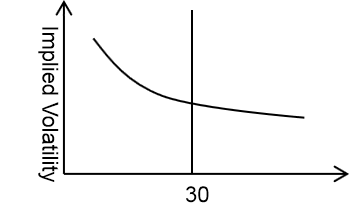
\includegraphics[width=0.5\textwidth]{images/1.png}
        \caption{示例图片}
        \label{fig:example}
    \end{figure}

    Assuming that the implied volatility at USD 50 is used to conduct the valuation, which of the following long positions will be undervalued?
    \\    一位风险管理师正在对一只当前价格为50美元的ABC非分红股票的多个欧式期权头寸进行估值。使用Black-Scholes-Merton模型和ABC股票在不同执行价格下活跃交易的欧式期权的当前价格估计的隐含波动率偏斜如下：

    \begin{figure}[H]
        \centering
        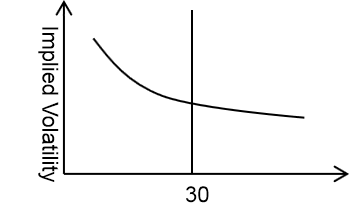
\includegraphics[width=0.5\textwidth]{images/1.png}
        \caption{示例图片}
        \label{fig:example}
    \end{figure}

    假设使用50美元的隐含波动率进行估值，以下哪些多头头寸将被低估？
    
\end{question}

\begin{choices}
    \item An out-of-the-money call
    \\ 价外看涨期权
    \item An in-the-money call
    \\ 价内看涨期权
    \item An at-the-money put
    \\ 平价看跌期权
    \item An in-the-money put
    \\ 价内看跌期权
\end{choices}

\begin{correctanswer}
    B
\end{correctanswer}

\begin{explanation}
    \textbf{A选项错误。}
    \begin{itemize}
        \item 价外看涨期权的行权价格高于50，其隐含波动率低于平价波动率，使用平价波动率会导致高估而不是低估。
    \end{itemize}
    
    \textbf{B选项正确。}
    \begin{itemize}
        \item 价内看涨期权的行权价格低于50，其隐含波动率高于平价波动率。使用平价波动率会导致期权价值被低估。
    \end{itemize}
    
    \textbf{C选项错误。}
    \begin{itemize}
        \item 平价看跌期权的行权价格等于50，使用平价波动率进行估值是准确的，不会产生低估。
    \end{itemize}
    
    \textbf{D选项错误。}
    \begin{itemize}
        \item 价内看跌期权的行权价格高于50，其隐含波动率低于平价波动率，使用平价波动率会导致高估而不是低估。
    \end{itemize}
\end{explanation}

\checklist{期权定价中的波动率微笑}

\begin{question}
    With all other things being equal, a risk monitoring system that assumes constant volatility for equity returns will understate the implied volatility for which of the following positions by the largest amount:
    \\ 在所有其他条件相同的情况下，假设股票收益率的波动率恒定的风险监控系统会对以下哪些头寸的隐含波动率低估最大？
\end{question}

\begin{choices}
    \item Short position in an at-the-money call
    \\ 平价看涨期权的空头头寸
    \item Long position in an at-the-money call
    \\ 平价看涨期权的多头头寸
    \item Short position in a deep out-of-the-money call
    \\ 深度价外看涨期权的空头头寸
    \item Long position in a deep in-the-money call
    \\ 深度价内看涨期权的多头头寸
\end{choices}

\begin{correctanswer}
    D
\end{correctanswer}

\begin{explanation}
    \textbf{A选项错误。}
    \begin{itemize}
        \item 平价看涨期权的隐含波动率与假设的恒定波动率差异较小，因此低估程度也较小。
    \end{itemize}
    
    \textbf{B选项错误。}
    \begin{itemize}
        \item 平价看涨期权的隐含波动率与假设的恒定波动率差异较小，因此低估程度也较小。
    \end{itemize}
    
    \textbf{C选项错误。}
    \begin{itemize}
        \item 深度价外看涨期权的隐含波动率通常低于平价期权，使用恒定波动率会导致高估而不是低估。
    \end{itemize}
    
    \textbf{D选项正确。}
    \begin{itemize}
        \item 深度价内看涨期权的隐含波动率显著高于平价期权。当风险监控系统假设恒定波动率时，会最大程度地低估这类期权的隐含波动率。
    \end{itemize}
\end{explanation}

\checklist{恒定波动率假设下的隐含波动率低估}


\begin{question}
    Michael Chen, FRM, is a hedge fund manager who is explaining implied volatility for currency options to junior analysts. Which of the following statements best completes his explanation?
    \\ Michael Chen, FRM，是一位对冲基金经理，正在向初级分析师解释货币期权的隐含波动率。以下哪项陈述最好地完成了他的解释？
\end{question}

\begin{choices}
    \item There is a greater chance of extreme price movements than predicted by a lognormal distribution
    \\ 存在比对数正态分布预测的更大概率的极端价格变动
    \item Arbitrage opportunities clearly exist
    \\ 套利机会显然存在
    \item The implied volatility of currency options is expected to increase in the near future
    \\ 货币期权的隐含波动率预计在未来短期内会增加
    \item There are no arbitrage opportunities unless the implied volatility versus strike price represents a skewness that is referred to as a smirk rather than a smile
    \\ 除非隐含波动率与行权价格的关系表现为偏斜，而不是微笑，否则不存在套利机会
\end{choices}

\begin{correctanswer}
    A
\end{correctanswer}

\begin{explanation}
    \textbf{A选项正确。}
    \begin{itemize}
        \item 如果货币期权的价外期权隐含波动率高于平价期权，这表明交易者认为极端价格变动的概率大于对数正态分布预测的概率。实证研究支持这一假设。
    \end{itemize}
    
    \textbf{B选项错误。}
    \begin{itemize}
        \item 波动率微笑现象本身并不表明存在套利机会。市场参与者对极端价格变动的预期差异是导致波动率微笑的原因。
    \end{itemize}
    
    \textbf{C选项错误。}
    \begin{itemize}
        \item 波动率微笑是描述隐含波动率与行权价格关系的静态特征，而不是对未来波动率变化的预测。
    \end{itemize}
    
    \textbf{D选项错误。}
    \begin{itemize}
        \item 波动率微笑和波动率偏斜（smirk）都是市场对极端价格变动预期的反映，与套利机会的存在与否无关。
    \end{itemize}
\end{explanation}

\checklist{货币期权波动率微笑与极端价格变动预期}


\begin{question}
    David Wang, FRM, uses the Black-Scholes-Merton (BSM) model to value options. Following the financial crisis of 2008-2010, he is more aware of the limitations of the BSM option pricing model. Which of the following statements best characterizes a major limitation of the BSM option pricing model?
    \\ David Wang, FRM，使用Black-Scholes-Merton (BSM)模型为期权定价。在2008-2010年的金融危机之后，他更加意识到BSM期权定价模型的局限性。以下哪项陈述最好地描述了BSM期权定价模型的主要局限性？
\end{question}

\begin{choices}
    \item The BSM model assumes strike prices have non-constant volatility
    \\ BSM模型假设行权价格具有非恒定的波动率
    \item Option traders often use a volatility smile with lower volatilities for out-of-the-money call and put options when applying the BSM model
    \\ 期权交易员通常在应用BSM模型时，对价外看涨期权和看跌期权使用较低的波动率，形成波动率微笑现象。
    \item For up-and-out calls and puts, the BSM model is insensitive to changes in implied volatility when the knock-out strike price is equal to the strike price and the interest rate equals the underlying asset return
    \\ 对于上升出局期权和看跌期权，BSM模型对隐含波动率的变化不敏感，当敲出价格等于行权价格且利率等于标的资产收益率时。
    \item For down-and-out calls and puts, the BSM model is insensitive to changes in option maturity when the knock-out strike price is greater than the strike price and the interest rate is greater than the underlying asset return
    \\ 对于下降出局期权和看跌期权，BSM模型对期权期限的变化不敏感，当敲出价格大于行权价格且利率大于标的资产收益率时。
\end{choices}

\begin{correctanswer}
    C
\end{correctanswer}

\begin{explanation}
    \textbf{A选项错误。}
    \begin{itemize}
        \item BSM模型实际上假设波动率是恒定的，而不是非恒定的。这是模型的一个基本假设。
    \end{itemize}
    
    \textbf{B选项错误。}
    \begin{itemize}
        \item 期权交易员通常对价外期权使用更高的波动率，而不是更低的波动率，这形成了波动率微笑现象。
    \end{itemize}
    
    \textbf{C选项正确。}
    \begin{itemize}
        \item 对于上升出局期权，当敲出价格等于行权价格且利率等于标的资产收益率时，BSM模型对隐含波动率的变化不敏感。这是模型的一个重要局限性。
    \end{itemize}
    
    \textbf{D选项错误。}
    \begin{itemize}
        \item 对于下降出局期权，BSM模型对期权期限的变化是敏感的，特别是在敲出价格大于行权价格且利率大于标的资产收益率的情况下。
    \end{itemize}
\end{explanation}

\checklist{BSM 模型在处理障碍期权（特别是上升出局期权）时的局限性}

\begin{question}
    An European call with a market price of \$3.5 has a BSM price of \$4.5. All else equal, the BSM price of a European put is \$2.5. What is the market price of the put?
    \\ 一个市场价格为\$3.5的欧式看涨期权的BSM价格为\$4.5。所有其他条件相同，一个欧式看跌期权的BSM价格为\$2.5。这个看跌期权的市
\end{question}

\begin{choices}
    \item \$2
    \item \$2.5
    \item \$1.5
    \item \$1
\end{choices}

\begin{correctanswer}
    C
\end{correctanswer}

\begin{explanation}
    \textbf{步骤1：理解看涨-看跌期权平价关系}
    \begin{itemize}
        \item 看涨-看跌平价关系：$C - P = S - Ke^{-rT}$
        \item 该关系对市场价格和BSM模型价格都成立。
        \item 如果市场价格与BSM价格存在差异，这种差异在平价关系两边应该保持一致。
    \end{itemize}

    \textbf{步骤2：建立平价关系一致性}
    \begin{itemize}
        \item 市场价格差异应等于BSM价格差异：
        \[
        C_{\text{mkt}} - C_{\text{BSM}} = P_{\text{mkt}} - P_{\text{BSM}}
        \]
        \item 已知：$C_{\text{mkt}} = \$3.5$，$C_{\text{BSM}} = \$4.5$，$P_{\text{BSM}} = \$2.5$
    \end{itemize}

    \textbf{步骤3：计算看跌期权的市场价格}
    \begin{itemize}
        \item 代入数值：
        \[
        3.5 - 4.5 = P_{\text{mkt}} - 2.5
        \]
        \[
        -1 = P_{\text{mkt}} - 2.5
        \]
        \[
        P_{\text{mkt}} = 2.5 - 1 = \$1.5
        \]
    \end{itemize}
\end{explanation}

\checklist{看涨-看跌期权平价关系}

\begin{question}
    Lisa, the Risk Market Analyst, calculated implied volatilities based on call options for Apple's traded equity. As it turns out, the shape of the corresponding implied volatility skew is somewhat typical of equity options; i.e., downward sloping per decreasing implied volatility as a function of increasing strike price. She draws the following conclusions:
    \begin{itemize}
 \item I.The implied distribution of Apple's stock price has negative skew and negative excess kurtosis.
\item II.For identical maturities, an in-the-money call (ITM call) option on Apple's stock is more expensive than an out-of-the-money put (OTM put) option.
\item III.Compared to the normal distribution, the implied distribution of Apple's stock price has a lighter left tail.
\item IV.Compared to the lognormal distribution, the implied distribution of Apple's stock price has a lighter right tail.
    \end{itemize}
 
    Which of her above conclusions is necessarily true?
    \\ 风险市场分析师Lisa基于苹果公司交易股票的看涨期权计算了隐含波动率。结果表明，相应的隐含波动率偏斜的形状在某种程度上是股票期权的典型特征；即，随着执行价格的增加，隐含波动率递减，呈向下倾斜。她得出以下结论：
    \begin{itemize}
 \item I.苹果公司股票价格的隐含分布具有负偏度和负超额峰度。
\item II.对于相同的到期日，苹果公司股票的实值看涨期权（ITM看涨期权）比虚值看跌期权（OTM看跌期权）更昂贵。
\item III.与正态分布相比，苹果公司股票价格的隐含分布具有更轻的左尾。
\item IV.与对数正态分布相比，苹果公司股票价格的隐含分布具有更轻的右尾。
    \end{itemize}
 
    她的上述结论中哪一个是必然正确的？
\end{question}

\begin{choices}
    \item None
    \item I only
    \item IV only
    \item II and III only
\end{choices}

\begin{correctanswer}
    C
\end{correctanswer}

\begin{explanation}
     \textbf{结论I：错误。}
        \begin{itemize}
            \item 向下倾斜的波动率偏斜（执行价格↑，隐含波动率↓）表明隐含分布具有负偏度（negative skew）。
            \item 但股票期权通常具有正超额峰度（positive excess kurtosis），即厚尾特征，而非负超额峰度。
            \item 因此结论I的后半部分错误。
        \end{itemize}

     \textbf{结论II：错误。}
        \begin{itemize}
            \item 价内看涨期权与价外看跌期权的价格比较取决于执行价格、标的资产价格、时间价值等多个因素。
            \item 不能断言价内看涨一定比价外看跌更贵。
        \end{itemize}

     \textbf{结论III：错误。}
        \begin{itemize}
            \item 向下倾斜的波动率偏斜表明市场对大幅下跌的担忧（更高的下跌概率）。
            \item 因此隐含分布的左尾通常比正态分布更重（更厚），而非更轻。
        \end{itemize}

     \textbf{结论IV：正确。}
        \begin{itemize}
            \item 向下倾斜的波动率偏斜表明市场对大幅上涨的预期较低。
            \item 因此隐含分布的右尾比对数正态分布更轻（更薄），反映市场认为大幅上涨的概率较低。
        \end{itemize}

\end{explanation}

\checklist{股票期权波动率微笑与期望短缺（ES）}


\begin{question}
    A committee of risk management practitioner discusses the difference between pricing deep out-of-the-money call options on TSLA stock and pricing deep out-of-the-money call options on the USD/CNY foreign exchange rate using the Black-Scholes-Merton (BSM) model. The practitioners price these options based on two distinct probability distributions of underlying asset prices at the option expiration date:
    \begin{itemize}
        \item A lognormal probability distribution
        \item An implied risk-neutral probability distribution obtained from the volatility smile for options of the same maturity
    \end{itemize}
    Using the lognormal instead of the implied risk-neutral probability distribution will tend to:
    \\    风险管理从业者委员会讨论使用Black-Scholes-Merton（BSM）模型对TSLA股票的深度虚值看涨期权和USD/CNY外汇汇率的深度虚值看涨期权进行定价的差异。从业者基于期权到期日标的资产价格的两种不同概率分布对这些期权进行定价：
    \begin{itemize}
        \item 对数正态概率分布
        \item 从相同到期日期权的波动率微笑中获得的隐含风险中性概率分布
    \end{itemize}
    使用对数正态分布而不是隐含风险中性概率分布将倾向于：
    
\end{question}

\begin{choices}
    \item Price the option on TSLA relatively high and price the option on USD/CNY relatively low
    \\ TSLA股票的深度虚值看涨期权相对较高，USD/CNY外汇汇率的深度虚值看涨期权相对较低
    \item Price the option on TSLA relatively low and price the option on USD/CNY relatively high
    \\ TSLA股票的深度虚值看涨期权相对较低，USD/CNY外汇汇率的深度虚值看涨期权相对较高
    \item Price the option on TSLA relatively low and price the option on USD/CNY relatively low
    \\ TSLA股票的深度虚值看涨期权相对较低，USD/CNY外汇汇率的深度虚值看涨期权相对较低
    \item Price the option on TSLA relatively high and price the option on USD/CNY relatively high
    \\ TSLA股票的深度虚值看涨期权相对较高，USD/CNY外汇汇率的深度虚值看涨期权相对较高
\end{choices}

\begin{correctanswer}
    A
\end{correctanswer}

\begin{explanation}
    \textbf{A选项正确。}
    \begin{itemize}
        \item 股票期权的隐含分布比对数正态分布有更重的左尾和更轻的右尾，因此使用对数正态分布会导致深度价外看涨期权被高估。
        \item 货币期权的隐含分布比对数正态分布有更重的尾部，因此使用对数正态分布会导致深度价外看涨期权被低估。
    \end{itemize}
    
\end{explanation}

\checklist{股票期权定价中的波动率微笑与期望短缺（ES）}


\begin{question}
    You are asked to mark to market a book of plain-vanilla stock options. The trader is short deep out-of-the-money options and long at-the-money options. There is a pronounced smile for these options. The trader's bonus increases as the value of his book increases. Which approach should you use to mark the book?
    \\ 你被要求对一揽子普通股票期权进行估值。交易员持有深度价外期权空头头寸和平价期权多头头寸。这些期权表现出明显的波动率微笑。交易员的奖金随着其头寸价值的增加而增加。你应该使用哪种方法来估值？
\end{question}

\begin{choices}
    \item Use the implied volatility of at-the-money options because the estimation of the volatility is more reliable
    \\ 使用平价期权的隐含波动率，因为隐含波动率的估计更可靠
    \item Use the average of the implied volatilities for the traded options for which you have data because it provides a balanced view
    \\ 使用交易期权的平均隐含波动率，因为它提供了平衡的视角
    \item For each option, use the implied volatility of the most similar option traded on the market
    \\ 对每个期权，使用市场上最相似期权的隐含波动率
    \item Use the historical volatility because doing so corrects for the pricing mistakes in the option mark
    \\ 使用历史波动率，因为它纠正了期权定价中的错误
\end{choices}

\begin{correctanswer}
    C
\end{correctanswer}

\begin{explanation}
    \textbf{A选项错误。}
    \begin{itemize}
        \item 使用平价期权的隐含波动率会低估价外期权的价值，这会人为地增加交易员的利润，不符合公允定价原则。
    \end{itemize}
    
    \textbf{B选项错误。}
    \begin{itemize}
        \item 使用平均隐含波动率会忽略波动率微笑的特征，无法准确反映不同行权价格期权的实际市场价值。
    \end{itemize}
    
    \textbf{C选项正确。}
    \begin{itemize}
        \item 对每个期权使用市场上最相似期权的隐含波动率，可以最准确地反映其市场价值。这种方法考虑了波动率微笑的特征，能够给出最接近市场价格的估值。
    \end{itemize}
    
    \textbf{D选项错误。}
    \begin{itemize}
        \item 历史波动率无法反映当前市场对未来价格变动的预期，不适合用于期权定价。
    \end{itemize}
\end{explanation}

\checklist{期权定价中的波动率微笑}

\begin{question}
    Suppose that a central bank's policy is to allow an exchange rate to fluctuate between 0.95 and 1.05. What pattern of implied volatilities for options on the exchange rate would you expect to see?
    \\ 假设一个中央银行的政策是允许汇率在0.95和1.05之间波动。你预计汇率期权的隐含波动率会呈现出哪种模式？
\end{question}

\begin{choices}
    \item    \begin{figure}[H]
        \centering
        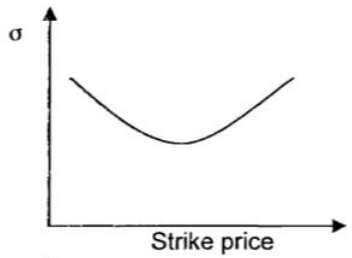
\includegraphics[width=0.2\textwidth]{images/A.png}
        \label{fig:example}
    \end{figure}
    \item    \begin{figure}[H]
        \centering
        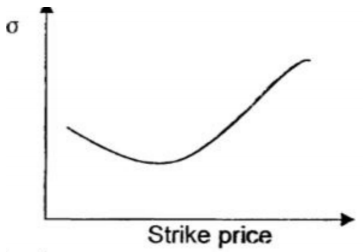
\includegraphics[width=0.2\textwidth]{images/B.png}
        \label{fig:example}
    \end{figure}
    \item    \begin{figure}[H]
        \centering
        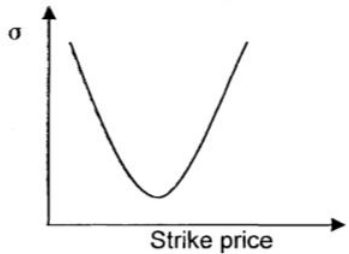
\includegraphics[width=0.2\textwidth]{images/C.png}
        \label{fig:example}
    \end{figure}
    \item    \begin{figure}[H]
        \centering
        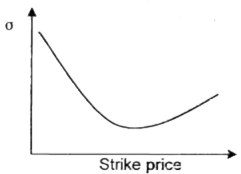
\includegraphics[width=0.2\textwidth]{images/D.png}
        \label{fig:example}
    \end{figure}
\end{choices}

\begin{correctanswer}
    A
\end{correctanswer}

\begin{explanation}
    \textbf{A选项正确。}
    \begin{itemize}
        \item 由于汇率波动范围被限制在0.95到1.05之间，这意味着汇率的最小值为0.95，最大值为1.05。与对数正态分布相比，汇率的隐含概率分布有更薄的左尾和右尾。因此，价外和价内期权的隐含波动率低于平价期权。
    \end{itemize}
    
    \textbf{B选项错误。}
    \begin{itemize}
        \item 这个选项显示的是波动率微笑，表示价外期权的隐含波动率高于平价期权，这与汇率波动范围限制的情况不符。
    \end{itemize}
    
    \textbf{C选项错误。}
    \begin{itemize}
        \item 这个选项显示的是波动率偏斜，表示低行权价格期权的隐含波动率高于高行权价格期权，这与汇率波动范围限制的情况不符。
    \end{itemize}
    
    \textbf{D选项错误。}
    \begin{itemize}
        \item 这个选项显示的是波动率frown（倒微笑），表示平价期权的隐含波动率高于价外期权，这与汇率波动范围限制的情况不符。
    \end{itemize}
\end{explanation}

\checklist{汇率期权波动率微笑}


\begin{question}
    An empirical distribution of equity price derived from the price of options of such stock based on BSM that exhibits a fatter right tail than that of a lognormal distribution would indicate:
    \\ 基于BSM模型对某股票期权价格得出的股票价格经验分布，其右尾比对数正态分布更厚，这表明：
\end{question}

\begin{choices}
    \item Equal implied volatilities across low and high strike prices
    \\ 低行权价格和高中行权价格的隐含波动率相等
    \item Greater implied volatilities for low strike prices
    \\ 低行权价格的隐含波动率更高
    \item Greater implied volatilities for high strike prices
    \\ 高中行权价格的隐含波动率更高
    \item Higher implied volatilities for mid-range strike prices
    \\ 中行权价格的隐含波动率更高
\end{choices}

\begin{correctanswer}
    C
\end{correctanswer}

\begin{explanation}
    \textbf{A选项错误。}
    \begin{itemize}
        \item 如果隐含波动率在低行权价格和高行权价格之间相等，这表明隐含分布与对数正态分布相似，没有表现出厚尾特征。
    \end{itemize}
    
    \textbf{B选项错误。}
    \begin{itemize}
        \item 低行权价格期权的隐含波动率更高通常表明隐含分布有厚左尾，而不是厚右尾。
    \end{itemize}
    
    \textbf{C选项正确。}
    \begin{itemize}
        \item 具有厚右尾的隐含分布表明观察到高标的资产价格的概率增加，这会导致高行权价格期权的隐含波动率更高。
    \end{itemize}
    
    \textbf{D选项错误。}
    \begin{itemize}
        \item 中等行权价格期权的隐含波动率更高通常表明隐含分布有更厚的中间部分，而不是厚右尾。
    \end{itemize}
\end{explanation}

\checklist{汇率期权波动率微笑与期望短缺（ES）}

\begin{question}
    A newly hired junior derivatives pricing analyst at an investment bank is evaluating option contracts on the USD/JPY exchange rate. The analyst observes that the risk-free interest rate is 3\% in the US and 0.1\% in Japan and gathers the following information on four European-style at-the-money options:

    \begin{table}[H]
        \centering
        \begin{tabular}{|c|c|c|c|}
        \hline
        Option & Option type & Days to expiration & Option price \\
        \hline
        1 & Call & 30 & 2.15 \\
        \hline
        2 & Put & 30 & 1.82 \\
        \hline
        3 & Call & 90 & 3.85 \\
        \hline
        4 & Put & 90 & 3.65 \\
        \hline
        \end{tabular}
        \end{table}
    The analyst uses the Black-Scholes-Merton model to calculate the implied volatilities of the options.
    Assuming no arbitrage opportunities, which of the following would the analyst be correct to conclude about these options?
    \\    一家投资银行新聘用的初级衍生品定价分析师正在评估USD/JPY汇率的期权合约。分析师观察到美国的无风险利率为3\%，日本为0.1\%，并收集了以下四个欧式平值期权的信息：

    \begin{table}[H]
        \centering
        \begin{tabular}{|c|c|c|c|}
        \hline
        期权 & 期权类型 & 到期天数 & 期权价格 \\
        \hline
        1 & 看涨期权 & 30 & 2.15 \\
        \hline
        2 & 看跌期权 & 30 & 1.82 \\
        \hline
        3 & 看涨期权 & 90 & 3.85 \\
        \hline
        4 & 看跌期权 & 90 & 3.65 \\
        \hline
        \end{tabular}
        \end{table}
    分析师使用Black-Scholes-Merton模型计算期权的隐含波动率。
    假设不存在套利机会，分析师关于这些期权的以下哪项结论是正确的？
\end{question}

\begin{choices}
    \item The implied volatility of the options expiring in 90 days is higher than that of the options expiring in 30 days due to the interest rate differential between the two countries
    \\ 由于两国之间的利率差异，90天到期的期权的隐含波动率高于30天到期的期权
    \item Put-call parity does not hold for these currency options since the prices of the at-the-money call options are not equal to the prices of the at-the-money put options
    \\ 看涨-看跌期权平价关系不成立，因为平价看涨期权的价格不等于平价看跌期权的价格
    \item The implied volatility of the at-the-money put option expiring in 30 days is the same as the implied volatility of the at-the-money call option expiring in 30 days
    \\ 30天到期的平价看跌期权的隐含波动率与30天到期的平价看涨期权的隐含波动率相同
    \item The volatility smiles for options on the USD/JPY exchange rate display positive upward skewness since the at-the-money option prices clearly display a preference for calls over puts
    \\ 汇率期权的波动率微笑显示出正向的上偏斜，因为平价期权的价格明显显示出对看涨期权的偏好超过看跌期权
\end{choices}

\begin{correctanswer}
    C
\end{correctanswer}

\begin{explanation}
    \textbf{A选项错误。}
    \begin{itemize}
        \item 利率差异会影响期权价格，但不会直接影响隐含波动率。隐含波动率主要反映市场对未来价格波动的预期。
    \end{itemize}
    
    \textbf{B选项错误。}
    \begin{itemize}
        \item 看涨-看跌期权平价关系（Put-call parity）仍然成立。平价期权中看涨和看跌期权的价格不同是由于利率差异导致的，这并不违反平价关系。
    \end{itemize}
    
    \textbf{C选项正确。}
    \begin{itemize}
        \item 对于具有相同行权价格和到期日的欧式期权，看涨期权的隐含波动率总是等于看跌期权的隐含波动率。这是因为它们都反映了同一标的资产的价格波动预期。
    \end{itemize}
    
    \textbf{D选项错误。}
    \begin{itemize}
        \item 平价期权中看涨期权价格高于看跌期权价格是由于利率差异导致的，而不是波动率微笑的偏斜特征。
    \end{itemize}
\end{explanation}

\checklist{隐含波动率曲面与波动率期限结构}


\begin{question}
    A pharmaceutical company plans to announce the results of a clinical trial in three months, which is expected to cause the price of its stock to move sharply, either up or down. A hedge fund manager would like to take advantage of this event by establishing an options position. In preparation, the manager examines the volatility curves, volatility term structure, and volatility surface of the options on the stock. Which of the following is correct for the manager to find through this examination?
    \\ 一家制药公司计划在三个月内宣布一项临床试验的结果，预计会导致其股价大幅波动，无论是上涨还是下跌。对冲基金经理希望利用这一事件建立期权头寸。在准备阶段，经理检查了股票期权的波动率曲线、波动率期限结构和波动率曲面。经理通过这项检查可以得出以下哪项结论？
\end{question}

\begin{choices}
    \item The volatility surface will reflect implied volatilities being an increasing function of time to maturity, regardless of the shape of the volatility curves
    \\ 波动率曲面将反映隐含波动率随到期时间的增加而增加，无论波动率曲线的形状如何
    \item The volatility curve at each maturity will steepen as the time to maturity of the options increases, regardless of the shape of the volatility curves
    \\ 每个到期日的波动率曲线随着期权的到期时间增加而变得更加陡峭，无论波动率曲线的形状如何
    \item The volatility curves of short-dated options that mature after the event form a steep smile, while the volatility curves of options with longer-dated maturities are flat
    \\ 事件发生后到期的短期期权的波动率曲线形成陡峭的微笑，而到期时间较长的期权的波动率曲线是平坦的
    \item The volatility curves for options with maturities of three months or longer are frown-shaped and the term structure of implied volatility is a decreasing function of time to maturity
    \\ 三个月或更长时间到期的期权的波动率曲线呈frown形状，隐含波动率的期限结构是随时间到期的递减函数
\end{choices}

\begin{correctanswer}
    C
\end{correctanswer}

\begin{explanation}
    \textbf{A选项错误。}
    \begin{itemize}
        \item 波动率曲面不一定总是到期时间的增函数。在重大事件（如临床试验结果公布）前后，短期期权的隐含波动率可能会显著高于长期期权。
    \end{itemize}
    
    \textbf{B选项错误。}
    \begin{itemize}
        \item 波动率曲线的陡峭程度不一定随着到期时间的增加而增加。在重大事件前后，短期期权的波动率曲线可能会更陡峭。
    \end{itemize}
    
    \textbf{C选项正确。}
    \begin{itemize}
        \item 在重大事件（如临床试验结果公布）前后，短期期权的波动率曲线会形成陡峭的微笑，因为市场预期价格会有大幅波动。而长期期权的波动率曲线则相对平坦，因为事件的影响会随时间减弱。
    \end{itemize}
    
    \textbf{D选项错误。}
    \begin{itemize}
        \item 在重大事件前后，波动率曲线通常呈现微笑形状而不是frown形状，且短期期权的隐含波动率通常高于长期期权。
    \end{itemize}
\end{explanation}

\checklist{重大事件对期权波动率曲线的影响}


\begin{question}
    A foreign exchange (FX) options analyst at a dealer bank is examining historical daily changes in several FX rates. The analyst compiles these daily changes into distributions that are used to determine the prices of FX options, which shape the options' implied volatility curves. The analyst also compares the typical implied distribution for FX options with a lognormal distribution. Which of the following observations regarding the distribution of FX rate changes is correct for the analyst to make?
    \\ 一家银行的外汇期权分析师正在检查几种外汇汇率的历史每日变化。分析师将这些每日变化编译成分布，用于确定外汇期权的价格，从而塑造期权的隐含波动率曲线。分析师还比较了外汇期权的典型隐含分布与对数正态分布。分析师关于外汇汇率变化分布的以下哪项观察是正确的？
\end{question}

\begin{choices}
    \item The excess kurtosis in FX rate distribution leads to higher prices for deep out-of-the-money put options than the prices derived using the lognormal distribution
    \\ 外汇汇率分布的超额峰度导致深度价外看跌期权的价格高于使用对数正态分布计算的价格
    \item The lognormal distribution reflecting daily FX rate changes causes the implied volatility smile exhibited by foreign exchange options
    \\ 反映每日外汇汇率变化的对数正态分布导致外汇期权表现出隐含波动率微笑
    \item The negative skewness of FX rate distributions leads to higher implied volatilities for deep out-of-the-money put options than for deep out-of-the-money call options
    \\ 外汇汇率分布的负偏度导致深度价外看跌期权的隐含波动率高于深度价外看涨期权的隐含波动率
    \item Distributions of historical daily FX rate changes generally have fewer observations close to the mean and more observations in the tails than a lognormal distribution
    \\ 历史每日外汇汇率变化分布通常在均值附近有更少的观测值，而在尾部有更多的观测值，而不是对数正态分布
\end{choices}

\begin{correctanswer}
    A
\end{correctanswer}

\begin{explanation}
    \textbf{A选项正确。}
    \begin{itemize}
        \item 汇率分布的超额峰度（excess kurtosis）表明极端价格变动的概率高于对数正态分布。这导致深度价外看跌期权的价格高于使用对数正态分布计算的价格。
    \end{itemize}
    
    \textbf{B选项错误。}
    \begin{itemize}
        \item 对数正态分布本身不会导致波动率微笑。波动率微笑是由于实际分布与对数正态分布的差异（如超额峰度）导致的。
    \end{itemize}
    
    \textbf{C选项错误。}
    \begin{itemize}
        \item 货币期权的波动率微笑通常是对称的，深度价外看跌期权的隐含波动率不一定高于深度价外看涨期权。
    \end{itemize}
    
    \textbf{D选项错误。}
    \begin{itemize}
        \item 汇率变动的历史分布通常比对数正态分布有更多的均值附近观测值和更少的尾部观测值，而不是相反。
    \end{itemize}
\end{explanation}

\checklist{汇率分布的超额峰度与期权价格}



\begin{question}
    A financial analyst at a wealth management firm is using the Merton model to value the debt and the equity of NET, a digital media company. NET's capital structure consists of senior debt, subordinated debt, and equity. The analyst notices that the company currently faces financial difficulties, resulting in its total asset value being almost equal to the value of its senior debt. A manager at the wealth management firm informs the analyst that NET's asset volatility is likely to increase and that there is an equal probability of NET being acquired by a larger competitor or filing for bankruptcy. Assuming the manager's information is correct, what is the most likely valuation consequence for NET?
    \\ 一家财富管理公司的金融分析师正在使用Merton模型对NET（一家数字媒体公司）的债务和股权进行估值。NET的资本结构由高级债务、次级债务和股权组成。分析师注意到公司目前面临财务困难，导致其总资产价值几乎等于其高级债务的价值。财富管理公司的一名经理告知分析师，NET的资产波动率可能会增加，并且NET被更大竞争对手收购或申请破产的可能性是相等的。假设经理的信息正确，NET的估值最可能产生什么后果？
\end{question}

\begin{choices}
    \item The values of equity and subordinated debt will increase, but the value of senior debt will decrease
    \\ 权益和次级债务的价值将增加，但高级债务的价值将减少
    \item The values of equity and senior debt will increase, but the value of subordinated debt will decrease
    \\ 权益和高级债务的价值将增加，但次级债务的价值将减少
    \item The values of equity and senior debt will decrease, but the value of subordinated debt will increase
    \\ 权益和高级债务的价值将减少，但次级债务的价值将增加
    \item The value of equity will increase, but the values of senior debt and subordinated debt will decrease
    \\ 权益的价值将增加，但高级债务和次级债务的价值将减少
\end{choices}

\begin{correctanswer}
    A
\end{correctanswer}

\begin{explanation}
    \textbf{A选项正确。}
    \begin{itemize}
        \item 资产波动率增加和可能的收购或破产会导致权益和次级债务的价值增加，因为这两种情况都可能带来更高的回报。而高级债务的价值会下降，因为波动率增加增加了违约风险。
    \end{itemize}
    
    \textbf{B选项错误。}
    \begin{itemize}
        \item 高级债务的价值不会增加，因为资产波动率增加会增加违约风险，降低高级债务的价值。
    \end{itemize}
    
    \textbf{C选项错误。}
    \begin{itemize}
        \item 权益的价值不会下降，因为可能的收购或破产都可能带来更高的回报。
    \end{itemize}
    
    \textbf{D选项错误。}
    \begin{itemize}
        \item 次级债务的价值不会下降，因为可能的收购或破产都可能带来更高的回报。
    \end{itemize}
\end{explanation}

\checklist{资产波动率增加对公司价值的影响}






\end{document}